\documentclass[tikz,border=4pt]{standalone}
\usepackage{ctex}
\usepackage{amsmath}
\usetikzlibrary{arrows.meta}

% p8-02c: 一次函数斜率的几何意义——倾斜方向示意（k正递增，k负递减）
\begin{document}
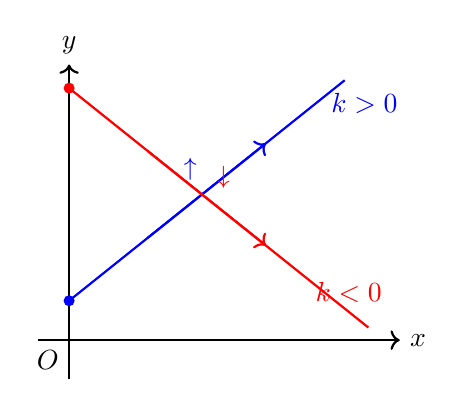
\begin{tikzpicture}[scale=1.0, thick]
  % 坐标轴
  \draw[->] (-0.4,0) -- (4.2,0) node[right] {$x$};
  \draw[->] (0,-0.5) -- (0,3.5) node[above] {$y$};
  \node[below left] at (0,0) {$O$};

  % k>0: y = 0.8x + 0.5（向右上倾）
  \draw[blue, thick] (0,0.5) -- (3.5, 3.3);
  \node[right, blue] at (3.2, 3.0) {$k>0$};
  % 标注"递增"方向箭头
  \draw[->, blue, thick] (1.0,1.3) -- (2.5,2.5) node[midway, above left] {\small$\uparrow$};

  % k<0: y = -0.8x + 3.2（向右下倾）
  \draw[red, thick] (0, 3.2) -- (3.8, 0.16);
  \node[right, red] at (3.0, 0.6) {$k<0$};
  % 标注"递减"方向箭头
  \draw[->, red, thick] (1.0,2.4) -- (2.5,1.2) node[midway, above right] {\small$\downarrow$};

  % 截距标注
  \fill[blue] (0,0.5) circle (2pt);
  \fill[red] (0,3.2) circle (2pt);
\end{tikzpicture}
\end{document}
